\documentclass[10pt,aspectratio=169]{beamer}
\usetheme{metropolis}
\usepackage{tikz}
\usepackage{xcolor}

\definecolor{nhsblue}{RGB}{0,94,184}
\definecolor{nhsgreen}{RGB}{0,177,64}

\begin{document}

\begin{frame}{Application Architecture}
\centering
\textbf{Four Key Modules:}

\vspace{0.5cm}
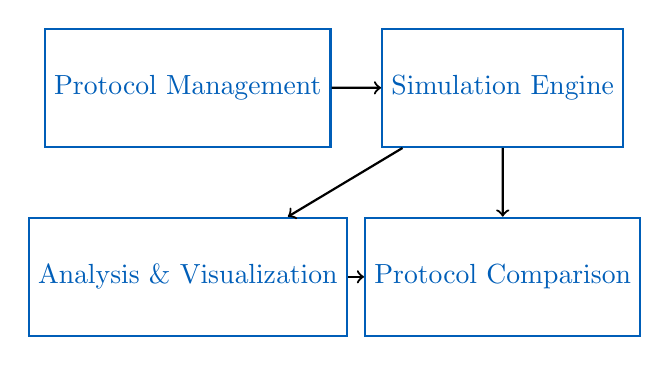
\begin{tikzpicture}[scale=0.8]
    \node[draw,nhsblue,thick,minimum width=3cm,minimum height=1.5cm] (proto) at (0,3) {Protocol Management};
    \node[draw,nhsblue,thick,minimum width=3cm,minimum height=1.5cm] (sim) at (5,3) {Simulation Engine};
    \node[draw,nhsblue,thick,minimum width=3cm,minimum height=1.5cm] (analysis) at (0,0) {Analysis \& Visualization};
    \node[draw,nhsblue,thick,minimum width=3cm,minimum height=1.5cm] (compare) at (5,0) {Protocol Comparison};
    
    \draw[->,thick] (proto) -- (sim);
    \draw[->,thick] (sim) -- (analysis);
    \draw[->,thick] (sim) -- (compare);
    \draw[->,thick] (analysis) -- (compare);
\end{tikzpicture}

\vspace{0.5cm}
\alert{Next: Live demonstration of the application}
\end{frame}

\end{document}